% =============================================================
% DIAGRAMA DE FLUJO: PROCESO DE BENEFICIO DEL CAFÉ
% Adaptado de: Borém (2008); Roa et al. (1999) – Cenicafé
% =============================================================


\usetikzlibrary{
    shapes.geometric,
    arrows.meta,
    positioning,
    fit,
    backgrounds,
    calc
}

% =============================================================
% COLORES
% =============================================================
\definecolor{cafeOscuro}{RGB}{101, 67, 33}
\definecolor{cafeClaro}{RGB}{210, 180, 140}
\definecolor{colorNatural}{RGB}{193, 120, 40}
\definecolor{colorHoney}{RGB}{160, 130, 10}
\definecolor{colorLavado}{RGB}{50, 110, 175}
\definecolor{colorComun}{RGB}{70, 125, 75}
\definecolor{colorDecision}{RGB}{130, 60, 150}
\definecolor{bgNatural}{RGB}{255, 243, 215}
\definecolor{bgHoney}{RGB}{255, 250, 210}
\definecolor{bgLavado}{RGB}{220, 238, 255}
\definecolor{bgComun}{RGB}{228, 244, 228}
\definecolor{bgDecision}{RGB}{245, 230, 250}

% =============================================================
% ESTILOS
% =============================================================
\tikzset{
    etapaComun/.style={
        rectangle, rounded corners=5pt,
        draw=colorComun, line width=1.1pt, fill=bgComun,
        text width=3.2cm, minimum height=0.9cm,
        align=center, font=\small\bfseries, text=cafeOscuro
    },
    decision/.style={
        diamond, aspect=2.6,
        draw=colorDecision, line width=1.1pt, fill=bgDecision,
        text width=2.4cm, align=center,
        font=\footnotesize\bfseries, text=colorDecision, inner sep=1pt
    },
    etapaNatural/.style={
        rectangle, rounded corners=5pt,
        draw=colorNatural, line width=1.1pt, fill=bgNatural,
        text width=2.4cm, minimum height=0.85cm,
        align=center, font=\small\bfseries, text=cafeOscuro
    },
    etapaHoney/.style={
        rectangle, rounded corners=5pt,
        draw=colorHoney, line width=1.1pt, fill=bgHoney,
        text width=2.4cm, minimum height=0.85cm,
        align=center, font=\small\bfseries, text=cafeOscuro
    },
    etapaLavado/.style={
        rectangle, rounded corners=5pt,
        draw=colorLavado, line width=1.1pt, fill=bgLavado,
        text width=2.4cm, minimum height=0.85cm,
        align=center, font=\small\bfseries, text=cafeOscuro
    },
    productoFinal/.style={
        rectangle, rounded corners=5pt,
        draw=cafeOscuro, line width=1.4pt, fill=cafeClaro,
        text width=3.2cm, minimum height=0.9cm,
        align=center, font=\small\bfseries, text=cafeOscuro
    },
    flechaComun/.style={
        -{Stealth[length=5pt,width=4pt]},
        line width=1.0pt, color=cafeOscuro
    },
    flechaNatural/.style={
        -{Stealth[length=5pt,width=4pt]},
        line width=1.0pt, color=colorNatural
    },
    flechaHoney/.style={
        -{Stealth[length=5pt,width=4pt]},
        line width=1.0pt, color=colorHoney
    },
    flechaLavado/.style={
        -{Stealth[length=5pt,width=4pt]},
        line width=1.0pt, color=colorLavado
    },
    labelSiNo/.style={
        font=\scriptsize\itshape, fill=white,
        inner sep=1.5pt, text=gray
    },
}

% =============================================================
\begin{document}

\begin{figure}[H]
\centering
\caption{Diagrama de flujo del proceso de beneficio del café
         (\textit{Coffea arabica} L.)}
\label{fig:diagrama_beneficio}
\vspace{0.3em}

% Coordenadas absolutas para control total del layout
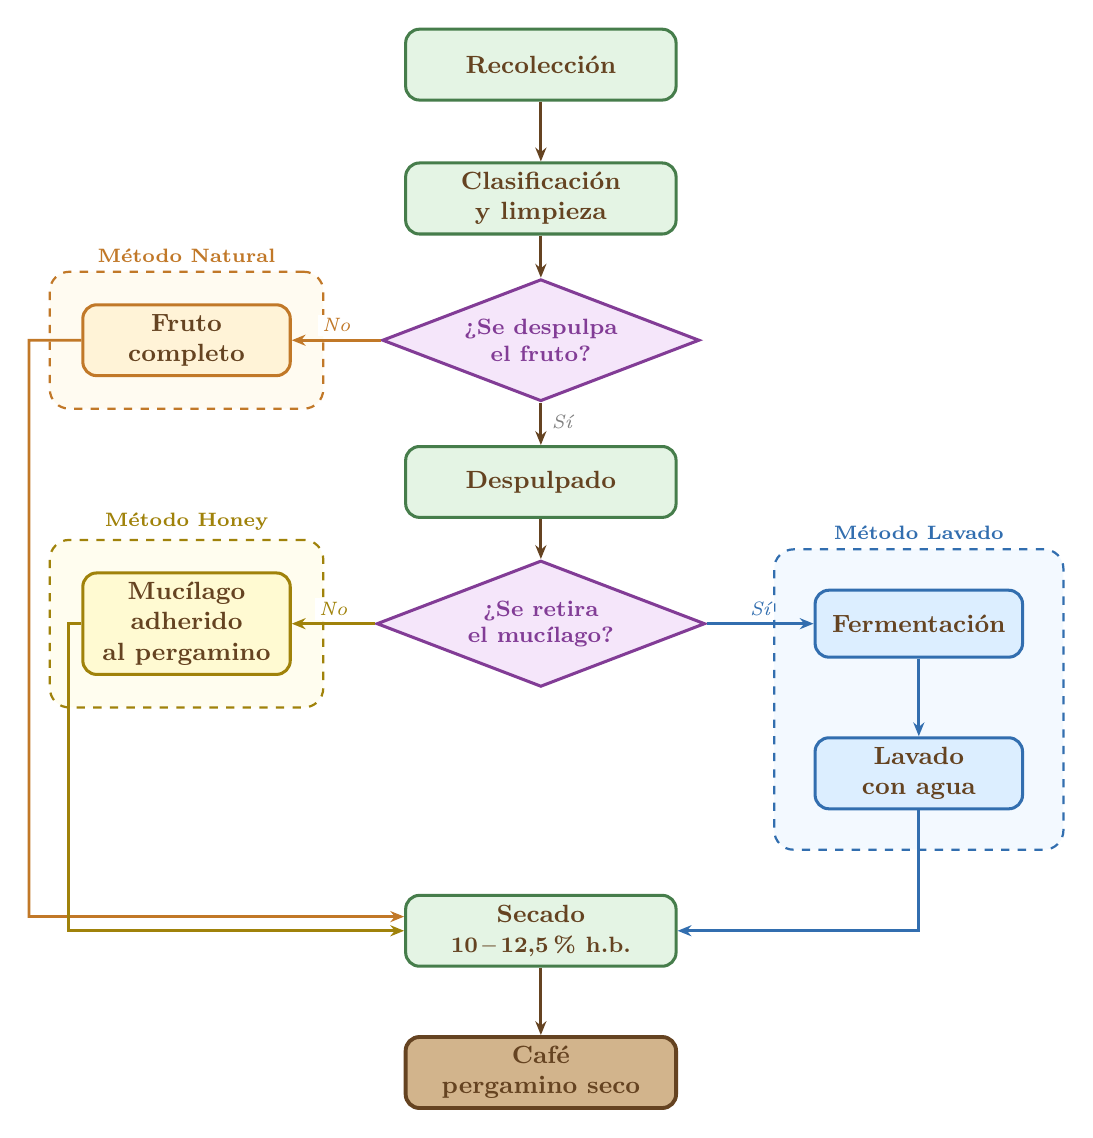
\begin{tikzpicture}[x=1cm, y=1cm]

    % ----------------------------------------------------------
    % NODOS — posiciones absolutas (xshift desde el centro = 0)
    % Eje central en x = 0
    % Rama izquierda centrada en x = -4.5
    % Rama derecha centrada en x = +4.8
    % ----------------------------------------------------------

    % Eje central
    \node[etapaComun]          at (0,  0.0) (recoleccion)  {Recolección};
    \node[etapaComun]          at (0, -1.7) (clasificacion){Clasificación y limpieza};
    \node[decision]            at (0, -3.5) (dec1)         {\footnotesize¿Se despulpa\\el fruto?};
    \node[etapaComun]          at (0, -5.3) (despulpado)   {Despulpado};
    \node[decision]            at (0, -7.1) (dec2)         {\footnotesize¿Se retira\\el mucílago?};
    \node[etapaComun]          at (0,-11.0) (secado)        {Secado\\{\footnotesize 10\,--\,12{,}5\,\% h.b.}};
    \node[productoFinal]       at (0,-12.8) (producto)     {Café pergamino seco};

    % Rama izquierda
    \node[etapaNatural]        at (-4.5, -3.5) (natural)   {Fruto completo};
    \node[etapaHoney]          at (-4.5, -7.1) (honey)     {Mucílago adherido\\al pergamino};

    % Rama derecha
    \node[etapaLavado]         at ( 4.8, -7.1) (fermentacion) {Fermentación};
    \node[etapaLavado]         at ( 4.8, -9.0) (lavadoAgua)   {Lavado con agua};

    % ----------------------------------------------------------
    % FLECHAS EJE CENTRAL
    % ----------------------------------------------------------
    \draw[flechaComun] (recoleccion)   -- (clasificacion);
    \draw[flechaComun] (clasificacion) -- (dec1);
    \draw[flechaComun] (dec1.south)    -- (despulpado.north)
        node[labelSiNo, pos=0.45, right=2pt]{Sí};
    \draw[flechaComun] (despulpado)    -- (dec2);
    \draw[flechaComun] (secado)        -- (producto);

    % ----------------------------------------------------------
    % BIFURCACIÓN 1 — Natural  (sale oeste de dec1)
    % ----------------------------------------------------------
    \draw[flechaNatural]
        (dec1.west) -- (natural.east)
        node[labelSiNo, midway, above=1pt,
             font=\scriptsize\itshape, text=colorNatural]{No};

    % ----------------------------------------------------------
    % BIFURCACIÓN 2 — Honey  (sale oeste de dec2)
    % ----------------------------------------------------------
    \draw[flechaHoney]
        (dec2.west) -- (honey.east)
        node[labelSiNo, midway, above=1pt,
             font=\scriptsize\itshape, text=colorHoney]{No};

    % ----------------------------------------------------------
    % BIFURCACIÓN 2 — Lavado  (sale este de dec2)
    % ----------------------------------------------------------
    \draw[flechaLavado]
        (dec2.east) -- (fermentacion.west)
        node[labelSiNo, midway, above=1pt,
             font=\scriptsize\itshape, text=colorLavado]{Sí};
    \draw[flechaLavado] (fermentacion) -- (lavadoAgua);

    % ----------------------------------------------------------
    % RUTAS HACIA SECADO
    %
    % NATURAL:
    %   natural.west → izquierda hasta x = -6.2
    %   baja hasta y = -11.0 (misma Y que secado)
    %   derecha hasta secado.west  (entra Y +0.18 arriba del centro)
    %
    % HONEY:
    %   honey.west → izquierda hasta x = -5.7  (distinto a -6.2)
    %   baja hasta y = -11.0
    %   derecha hasta secado.west  (entra justo en el centro)
    %
    % LAVADO:
    %   lavadoAgua.south → baja hasta y = -11.0
    %   izquierda hasta secado.east
    % ----------------------------------------------------------

    % ---- NATURAL ----
    % Segmentos: oeste → x=-6.2 | baja → y=-11.0+0.18 | este → secado.west+0.18
    \draw[flechaNatural]
        (natural.west)
        -- (-6.5, -3.5)
        -- (-6.5, -10.82)
        -- ($(secado.west) + (0, 0.18)$);

    % ---- HONEY ----
    % Segmentos: oeste → x=-5.7 | baja → y=-11.0 | este → secado.west
    \draw[flechaHoney]
        (honey.west)
        -- (-6.0, -7.1)
        -- (-6.0, -11.0)
        -- (secado.west);

    % ---- LAVADO ----
    % Segmentos: sur de lavadoAgua → y=-11.0 | oeste → secado.east
    \draw[flechaLavado]
        (lavadoAgua.south)
        -- (4.8, -11.0)
        -- ($(secado.east) + (0.4, 0)$)
        -- (secado.east);

    % ----------------------------------------------------------
    % RECUADROS PUNTEADOS + ETIQUETAS
    % ----------------------------------------------------------
    \begin{scope}[on background layer]
        \node[
            draw=colorNatural, line width=0.8pt,
            fill=bgNatural, fill opacity=0.35,
            dashed, rounded corners=7pt,
            fit=(natural), inner sep=0.4cm
        ] (boxNatural) {};

        \node[
            draw=colorHoney, line width=0.8pt,
            fill=bgHoney, fill opacity=0.35,
            dashed, rounded corners=7pt,
            fit=(honey), inner sep=0.4cm
        ] (boxHoney) {};

        \node[
            draw=colorLavado, line width=0.8pt,
            fill=bgLavado, fill opacity=0.35,
            dashed, rounded corners=7pt,
            fit=(fermentacion)(lavadoAgua), inner sep=0.5cm
        ] (boxLavado) {};
    \end{scope}

    \node[above=0.05cm of boxNatural,
          font=\scriptsize\bfseries, text=colorNatural,
          fill=white, inner sep=1.5pt] {Método Natural};

    \node[above=0.05cm of boxHoney,
          font=\scriptsize\bfseries, text=colorHoney,
          fill=white, inner sep=1.5pt] {Método Honey};

    \node[above=0.05cm of boxLavado,
          font=\scriptsize\bfseries, text=colorLavado,
          fill=white, inner sep=1.5pt] {Método Lavado};

\end{tikzpicture}

\vspace{0.4em}
\small\textit{Fuente: Adaptado de Borém (2008); Roa et al. (1999)
--- Cenicafé; Polakovicova et al. (2022).}

\end{figure}

\end{document}